\documentclass{article}
%\documentclass[conference]{IEEEtran}
%\usepackage[utf8]{inputenc}
\usepackage[margin=1.4in]{geometry}
\title{ZeRO: Memory Optimizations Toward Training Trillion Parameter Models}

\author{
    XXX \thanks{The original paper is located at \url{https://arxiv.org/abs/1910.02054}. This version has been modified by LuYF-Lemon-love <\url{luyanfeng_nlp@qq.com}> for personal study.}\\
    Microsoft
}

\date{}
\usepackage{xspace}
\usepackage{graphicx}
\usepackage{multirow}
\usepackage{hhline}
\usepackage{comment}
\usepackage{adjustbox}
\usepackage{xcolor}
\usepackage{pifont}
\usepackage{hyperref}
\usepackage{subcaption}
\usepackage{ulem}
\renewcommand{\baselinestretch}{1.0}
\usepackage[switch,columnwise]{lineno}

\newcommand{\name}{\textbf{ZeRO}\xspace}
\newcommand{\nameos}{\emph{ZeRO-OS}\xspace}

\newcommand{\mycheckmark}{\color{green} \ding{51}}
\newcommand{\mycrossout}{\color{red} \ding{55}}

\begin{document}

\maketitle
\section*{Abstract}
We develop a novel solution, Zero Redundancy Optimizer (\name), to optimize memory, vastly improving training speed while increasing the model size that can be efficiently trained.
\name eliminates memory redundancies in data- and model-parallel training while retaining low communication volume and high computational granularity, allowing us to scale the model size proportional to the number of devices with sustained high efficiency. Our analysis on memory requirements and communication volume demonstrates: \name has the potential to scale beyond 1 \emph{Trillion} parameters using today's hardware.

\section{Extended Introduction}
\label{sec:introduction}

\uline{MP splits the model vertically, partitioning the computation and parameters in each layer across multiple devices, requiring significant communication between each layer.} As a result, they work well within a single node where the inter-GPU communication bandwidth is high, but the efficiency degrades quickly beyond a single node \cite{megatronlm}.    

We first analyze the full spectrum of memory consumption of the existing systems on model training and classify it into two parts:  1) For large models, the majority of the memory is occupied by \emph{model states} which include \uline{the optimizer states} (such as momentum and variances in Adam~\cite{DBLP:journals/corr/Adam}), \uline{gradients}, and \uline{parameters}. 
2) The remaining memory is consumed by \uline{activation}, \uline{temporary buffers} and \uline{unusable fragmented memory}, which we refer to collectively as \emph{residual} states.
We develop \name --- Zero Redundancy Optimizer  --- to optimize memory efficiency on both while obtaining high compute and communication efficiency.

{\bf Optimizing Model State Memory:}
DP has good compute/communication efficiency but poor memory efficiency while MP can have poor compute/communication efficiency.
More specifically, \uline{DP replicates the entire model states across all data parallel process resulting in redundant memory consumption};
while \uline{MP partition these states to obtain high memory efficiency, but often result in too fine-grained computation and expensive communication that is less scaling efficient.}
Furthermore, all of these approaches maintain all the model states required over the entire
training process statically, even though not all model states are required all the time during
the training.

\textbf{\name-DP removes the memory state redundancies across data-parallel processes by \emph{partitioning} the model states instead of replicating them, and it retains the compute/communication efficiency by retaining the computational granularity and communication volume of DP using a dynamic communication schedule during training.}

\name-DP has three main optimization stages (as depicted in Figure \ref{fig:memory-consumption}), which correspond to the partitioning of optimizer states, gradients, and parameters. When enabled cumulatively:

\begin{figure}[t!]
 \begin{center}
 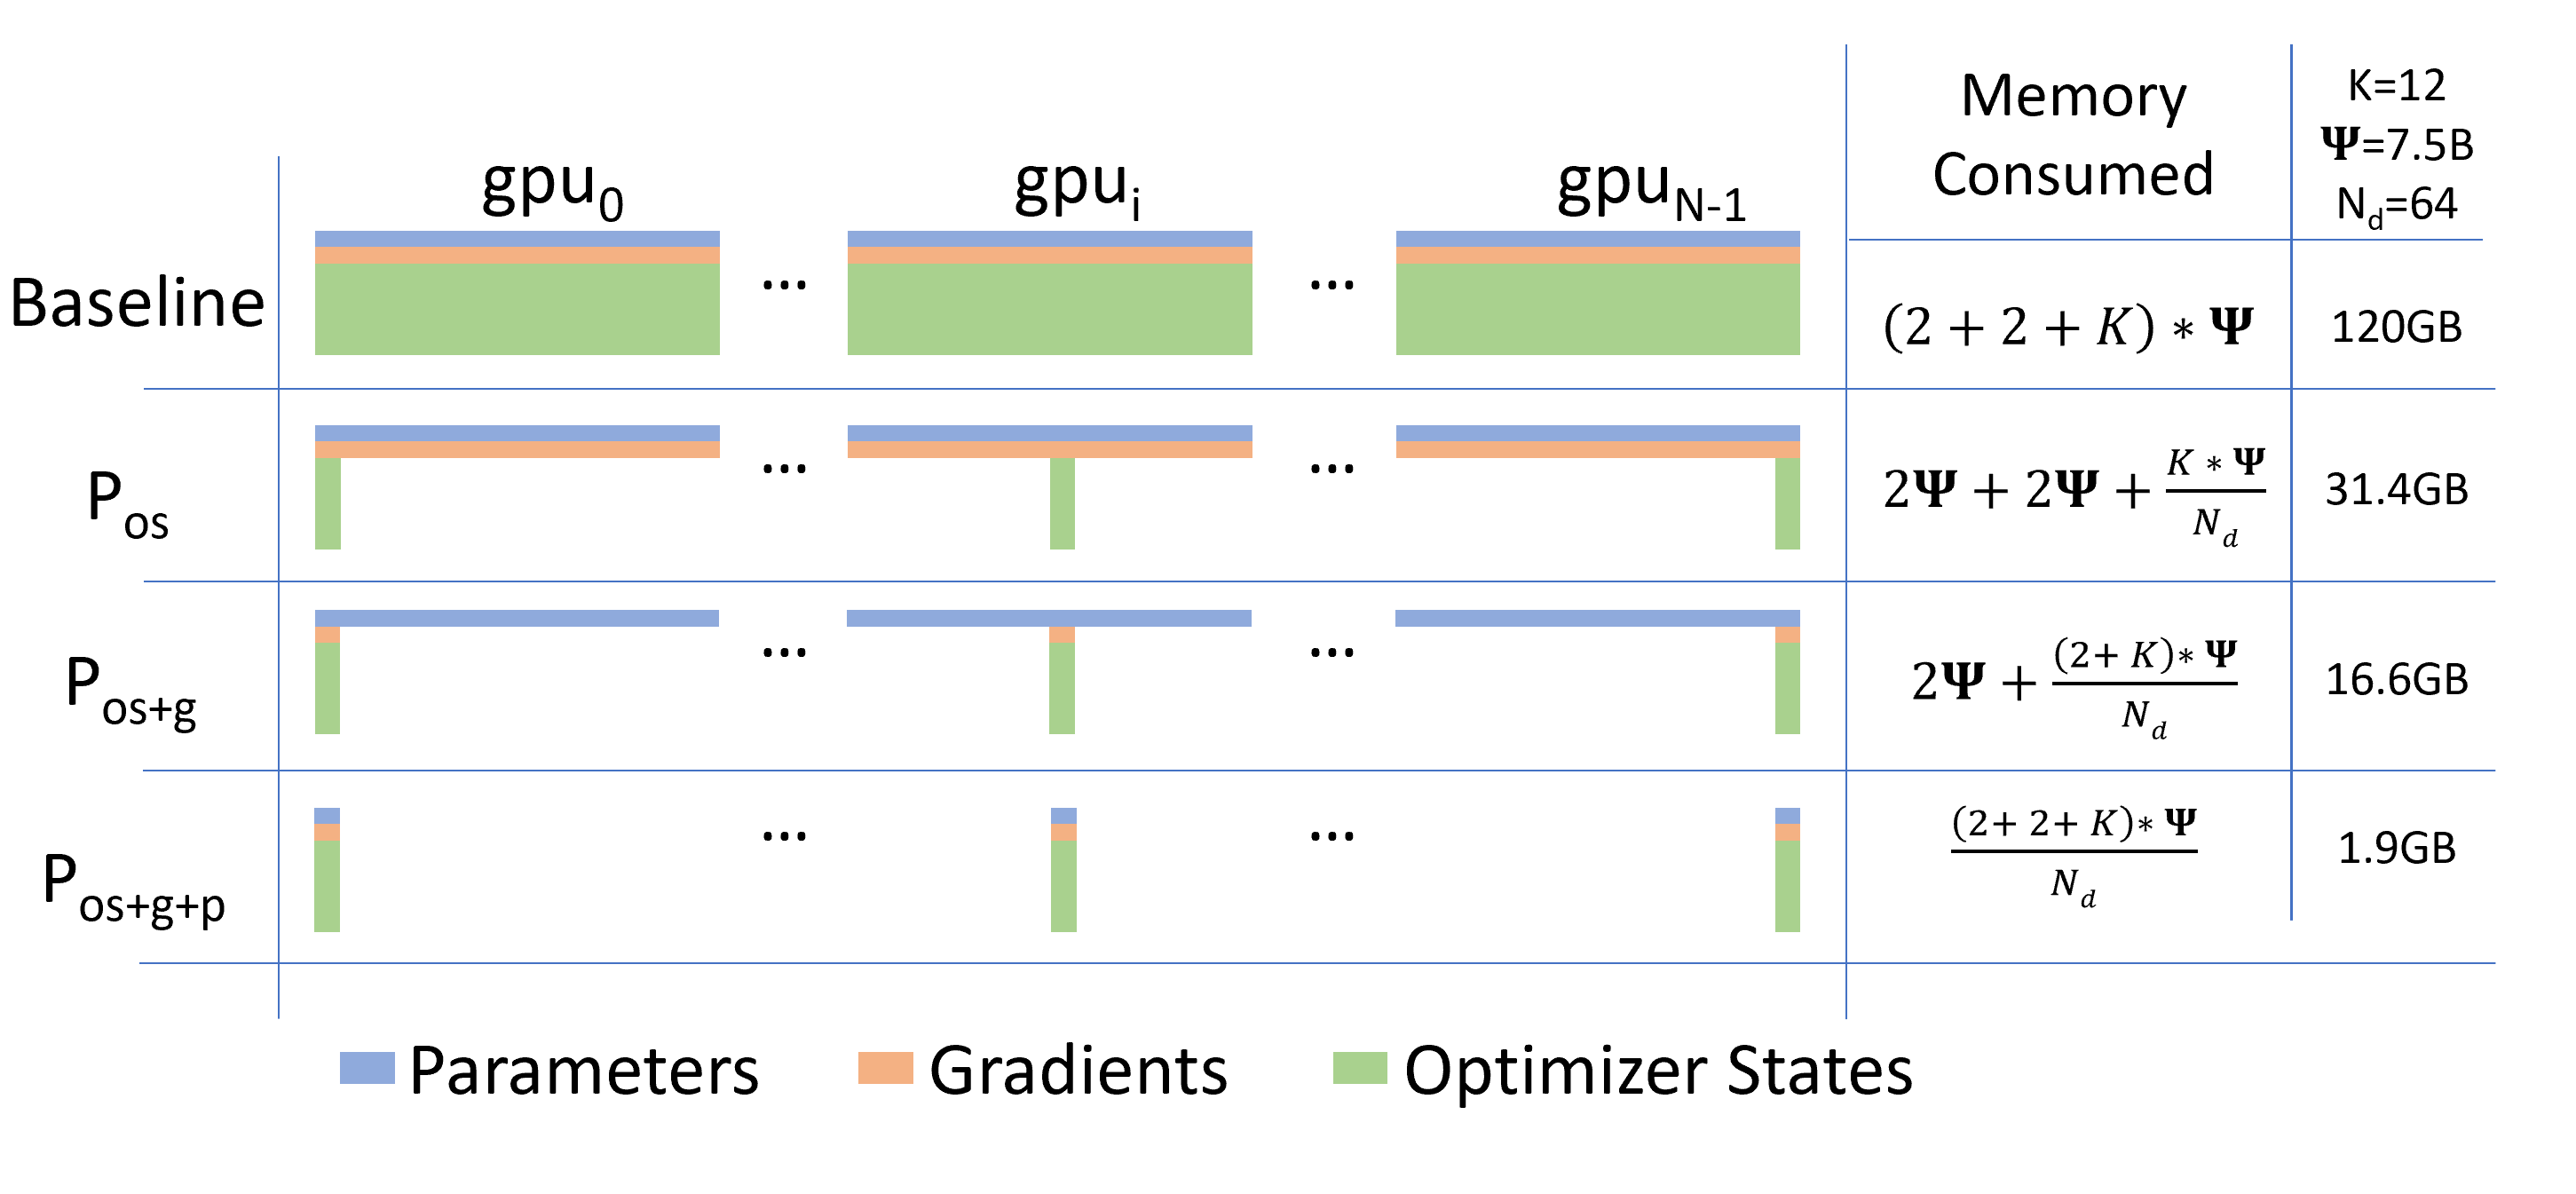
\includegraphics[width=1.0\columnwidth]{memory-consumption-v4.PNG}
 \caption{Comparing the per-device memory consumption of model states, with three stages of \name-DP optimizations. $\Psi$ denotes model size (number of parameters), $K$ denotes the memory multiplier of optimizer states, and $N_d$ denotes DP degree.  In the example, we assume a model size of $\Psi=7.5B$ and DP of $N_d=64$ with $K=12$ based on mixed-precision training with Adam optimizer. } 
 \label{fig:memory-consumption}
 \end{center}
\end{figure}

1) \uline{Optimizer State Partitioning ($P_{os}$): 4x memory reduction, same communication volume as DP;}

2) \uline{Add Gradient Partitioning ($P_{os+g}$): 8x memory reduction, same communication volume as DP;} 

3) \uline{Add Parameter Partitioning ($P_{os+g+p}$): Memory reduction is linear with DP degree $N_d$.} For example, splitting across 64 GPUs ($N_d$ = 64) will yield a 64x memory reduction. \uline{There is a modest 50\% increase in communication volume.}

{\bf Optimizing Residual State Memory:}
We develop \name-R to optimize the residual memory consumed by these three factors respectively.  

1) For activations (stored from forward pass in order to perform backward pass), we noticed checkpointing \cite{DBLP:journals/corr/ChenXZG16} helps but not sufficient for large models.  
\uline{Thus \name-R optimizes activation memory by identifying and removing activation replication in existing MP approaches through activation partitioning.} \uline{It also offloads activations to CPU when appropriate.}

2) \uline{\name-R defines appropriate size for temporary buffers to strike for a balance of memory and computation efficiency.}

3) We observe fragmented memory during training due to variations in the lifetime of different tensors. Lack of contiguous memory due to fragmentation can cause memory allocation failure, even when enough free memory is available. \uline{\name-R proactively manages memory based on the different lifetime of tensors, preventing memory fragmentation.}

\name-DP and \name-R combined together forms a powerful system of memory optimizations for DL training that we collectively refer to as \name.

There are still cases where we want to leverage MP: i) When used with \name-R, MP can reduce activation memory footprint for very large models. ii) For smaller models where activation memory is not an issue, MP can also have benefits when aggregated batch size using DP alone is too big to have good convergence.\footnote{Prior work \cite{DBLP:journals/corr/batch-scaling} shows, very large batch size could slow down convergence.  For given model and data, there is a measure of critical-batch size, where increasing batch size further slows down convergence.}  In those case, one can combine \name with MP to fit the model with an acceptable aggregated batch size.

We share \name as a part of our open source DL training optimization library called DeepSpeed\footnote{https://github.com/microsoft/deepspeed}.
\section{Related Work}
\label{sec:related-work}
\subsection{Data, Model and Pipeline Parallelism}
For a model that fits in the device memory for training, data parallelism (DP) is used to scale training to multiple devices. \uline{In DP, model parameters are replicated on each device. At each step, a mini-batch is divided evenly across all the data parallel processes, such that each process executes the forward and backward propagation on a different subset of data samples, and uses averaged gradients across processes to update the model locally.}

When a model does not fit in the device memory, model parallelism (MP) \cite{DBLP:journals/corr/mesh-tensor, megatronlm} and pipeline parallelism (PP) \cite{GPipe, DBLP:journals/corr/pipedream} split the model among processes, in vertical and horizontal way respectively.

PP splits a model horizontally across layers running each partition on a different device and use micro-batching to hide the pipeline bubble \cite{GPipe,DBLP:journals/corr/pipedream}.
\uline{Model functionalities such as tied-weights and batch-normalization are difficult to implement due to horizontal splitting and micro-batching, respectively.}

Popular PP implementation such as G-pipe \cite{GPipe} partitions both model parameters and total activations but requires a batch size proportional to number of pipeline partitions to hide the pipeline bubble.
\uline{The large batch size can affect the convergence rate, while also requiring significant memory to store activations.}

A different implementation of PP in PipeDream \cite{narayanan2019pipedream} keeps multiple copies of stale parameters to hide the pipeline bubble without increasing the batch size significantly, making it less memory efficient.
\uline{Additionally, the implementation is not equivalent to the standard DL training and has implications on training convergence.}

\subsection{Non-parallelism based approach to reduce memory}

\subsubsection{Reducing Activation Memory}

Multiple efforts have focused on reducing the memory footprint of activations through compression~\cite{jain2018gist}, activation checkpointing~\cite{DBLP:journals/corr/ChenXZG16, Jain2019CheckmateBT}, or live analysis \cite{DBLP:journals/corr/abs-1801-04380}. \uline{These efforts are complimentary and can work together with \name.} \uline{In fact, activation memory reduction in \name-R works in parallel with activation checkpointing.}

\subsubsection{CPU Offload}

\cite{layer2layer, 7783721} exploit heterogeneous nature of today's compute nodes, offloading model states to CPU memory through algorithmic design or virtualized memory, respectively. Up to $50\%$ of training time can be spent on GPU-CPU-GPU transfers \cite{layer2layer}. \uline{\name differs in that it reduces the memory consumption significantly without storing the model states to CPU memory whose bandwidth is severely constrained due to PCI-E.} \uline{On rare cases, \name-R may offload just the activation checkpoints for very large models to improve performance (see Sec.~\ref{sec:p_a} for details).}

\subsubsection{Memory Efficient Optimizer}

\cite{DBLP:journals/corr/adafactor,Anil2019MemoryEfficientAO} focus on reducing memory consumption of adaptive optimization methods by maintaining coarser-grained statistics of model parameters and gradients, with potential impact on model convergence guarantees. \uline{\name is orthogonal to these efforts, and its optimizations 
do not change the model optimization method or affect model convergence, but effectively reduce memory footprint of optimizer states and gradients per device.}

\subsection{Training Optimizers }

Adaptive optimization methods~\cite{10.5555/Adagrad,DBLP:journals/corr/Adam,DBLP:journals/corr/You-LARS,DBLP:journals/corr/You-LAMB} are crucial to achieving SOTA performance and accuracy for effective model training of large models. \uline{Compared to SGD, by maintaining fine-grained first-order and second-order statistics for each model parameter and gradient at the cost of significant memory footprint.}
\section{Where Did All the Memory Go?}
Let's take a step back to examine the memory consumption of the current training system.  For example,  a 1.5B parameter GPT-2 model requires 3GB of memory for its weights (or parameters) in 16-bit precision, yet, it cannot be trained on a single GPU with 32GB memory using Tensorflow or PyTorch.  One may wonder where all the memory goes.
During model training, most of the memory is consumed by {\it model states}, i.e., tensors comprising of pptimizer states, gradients, and parameters. Besides these model states, the rest of the memory is consumed by activations, temporary buffers and fragmented memory which we call \emph{residual states}. We look at the memory consumption from both in details.
\begin{comment}
and iii) temporary buffers. It is possible to trivially  Here we look at the memory consumed by latter two of the three.
\end{comment}

\subsection{Model States: Optimizer States, Gradients and Parameters} Majority of the device memory is consumed by model states during training.  Consider for instance, Adam~\cite{DBLP:journals/corr/Adam}, one of the most popular optimizers for DL training. Adam requires storing two optimizer states, i) the time averaged momentum and ii) variance of the gradients to compute the updates. Therefore, to train a model with ADAM, there has to be enough memory to hold a copy of both the momentum and variance of the gradients. In addition, there needs to be enough memory to store the gradients and the weights themselves. Of these three types of the parameter-related tensors, the optimizer states usually consume the most memory, specially when mixed-precision training is applied.

\textbf{Mixed-Precision Training} The state-of-the-art approach to train large models on the current generation of NVIDIA GPUs is via mixed precision (fp16/32) training~\cite{micikevicius2017mixed}, where parameters and activations are stored as fp16, enabling the use of the high throughput tensor core units~\cite{nvidia-volta-arch} on these GPUs. During mixed-precision training, both the forward and backward propagation are performed using fp16 weights and activations. However, to effectively compute and apply the updates at the end of the backward propagation, the mixed-precision optimizer keeps an fp32 copy of the parameters as well as an fp32 copy of all the other optimizer states. 

Let's take Adam as a concrete example.  Mixed precision training of a model with $\Psi$ parameters using Adam requires enough memory to hold an $fp16$ copy of the parameters and the gradients, with memory requirements of $2\Psi$ and $2\Psi$ bytes respectively.  In addition, it needs to hold the optimizer states: an $fp32$ copy of the parameters, momentum and variance, with memory requirements of $4\Psi$, $4\Psi$, and $4\Psi$ bytes, respectively.  Let's use $K$ to denote the memory multiplier of the optimizer states, i.e., the additional memory required to store them is $K\Psi$ bytes. Mixed-precision Adam has $K=12$. In total, this results in $2\Psi + 2\Psi + K\Psi = 16\Psi$ bytes of memory requirement. 
For a model such as GPT-2 with $1.5$ Billion parameters, this leads to a memory requirement of at least $24\,GB$, which is significantly higher than the meager $3\,GB$ of memory required to hold the $fp16$ parameters alone.

\subsection{Residual Memory Consumption}
\textbf{Activations} can take up a significant amount of memory \cite{DBLP:journals/corr/ChenXZG16} during training.  As a concrete example, the 1.5B parameter GPT-2 model trained with sequence length of 1K and batch size of 32 requires about 60\,GB of memory\footnote{The activation memory of a transformer-based model is proportional to the number of transformer layers $\times$ hidden dimensions $\times$  sequence length $\times$ batch size.  For a GPT-2 like architecture the total activations is about  $12 \times hidden\_dim \times batch \times seq\_length \times transformer\_layers$.}.  Activation checkpointing (or activation recomputation) is a common approach to reduce the activation memory by approximately the square root of the total activations at the expense of $33\%$ re-computation overhead \cite{DBLP:journals/corr/ChenXZG16}. This would reduce the activation memory consumption of this model to about 8\,GB.

Despite the significant reduction, the activation memory can grow quite large for bigger models even with activation checkpointing. For example, a GPT-like model with 100 billion parameters requires around 60 GB of memory for batch size 32, even when using activation checkpointing.

\begin{comment}
the amount of activation memory for a transformer based language model is proportional to the batch size, sequence length, hidden dimension and the number of layers . 
Activations take a non-trivial amount of memory even when using techniques such as activation checkpointing which significantly reduce the memory required by the activations at the expense of a $33\%$ re-computation overhead\cite{}.


For example, lets consider the 1.5B parameter GPT-2 model. Without activation checkpointing a transformer model produces $O(\frac{model\_size}{hidden\_dim}*seq\_length*batch$) activation, while with activation checkpointing it produces $O(\frac{model\_size}{hidden\_dim}*seq\_length*batch$) activations if we stored the activations only at the transformer layer boundary. For a batch size of 32, the GPT-2 models will therefore produce about 60GB of activations in fp16, while with activation checkpointing, it produces about 5 GB of activations.
\end{comment}

\textbf{Temporary buffers} used for storing intermediate results consumes non-trivial amount of memory for large models.   Operations such as gradient all-reduce, or gradient norm computation tend to fuse all the gradients into a single flattened buffer before applying the operation in an effort to improve throughput. For example, the bandwidth of all-reduce across devices improves with large message sizes. While the gradient themselves are usually stored as fp16 tensors, the fused buffer can be an fp32 tensor depending on the operation. When the size of the model is large, these temporary buffer sizes are non-trivial. For example, for a model with 1.5B parameters, a flattened fp32 buffer would required $6\,GB$ of memory. 

\textbf{Memory Fragmentation: }  So far we have discussed the actual memory consumption during training. Additionally, it is possible to run out of usable memory even when there is plenty of available memory. This can happen with memory fragmentation. A request for a memory will fail if there isn't enough contiguous memory to satisfy it, even if the total available memory is larger than requested. We observe significant memory fragmentation when training very large models, resulting in out of memory issue with over 30\% of memory still available in some extreme cases.
\begin{comment}

Training a large model with many layers can runs out of memory during training, even when there is plenty of available memory. 

We find that activation checkpointing and backward propagation can cause heavy memory fragmentation, making significant portion of the GPU memory unusable, even when there is plenty of available memory. 
The memory fragmentation is caused by activation checkpointing and backward propagation allocating long term and shot term memory in an interleaved fashion. During the forward propagation, temporary buffers are created in between the creation of each activation checkpoint, causing memory fragmentation. Similarly, in backward propagation working memory is allocated between computation of the gradients, also causing memory fragmentation. We find that for models with hundreds of layers, memory fragmentation can make over 30\% of the GPU memory unusable.
\end{comment}


\section{\name: Insights and Overview}
\name has two sets of optimizations: i) \name-DP aimed at reducing the memory footprint of the model states, and ii) \name-R targeted towards reducing the residual memory consumption.

\subsection{Insights and Overview: \name-DP}
\name powered DP is based on three key insights:

{\it a)} DP has better scaling efficiency than MP because MP reduces the granularity of the computation while also increasing the communication overhead. \uline{Beyond a certain point, lower computational granularity reduces the efficiency per GPU, while the increased communication overhead, hiders the scalability across GPUs, especially when crossing node boundaries.} On the contrary, DP has both higher computational granularity and lower communication volume, allowing for much higher efficiency.

{\it b)} \uline{DP is memory inefficient as model states are stored redundantly across all data-parallel processes. On the contrary, MP partitions the model states to obtain memory efficiency.}

{\it c)} \uline{Both DP and MP keep all the model states needed over the entire training process, but not everything is required all the time.}  For example, parameters corresponding to each layer is only needed during the forward propagation and backward propagation of the layer.  

Based on these insights, \name-DP retains the training efficiency of DP while achieving the memory efficiency of MP. \uline{\name-DP \textbf{partitions} the model states instead of replicating them (Section \ref{sec:memoryoptimization}) and uses a dynamic communication schedule that exploits the intrinsically temporal nature of the model states while minimizing the communication volume (Section \ref{sec:communication}).} By doing so, \name-DP reduces per-device memory footprint of a model \textbf{linearly} with the increased DP degree while maintaining the communication volume close to that of the default DP, retaining the efficiency.

\subsection{Insights and Overview: \name-R}

\label{sec:mp_activation_replication}
\subsubsection{Reducing Activation Memory}

Two key insights are:

{\it a)} \uline{MP partitions the model states but often requires replication of the activation memory.} For example, if we split the parameters of a linear layer vertically and compute them in parallel across two GPUs, each GPU requires the entire activation to compute its partition

{\it b)} For models such as GPT-2 or larger, the arithmetic intensity (ratio of the amount of computation per iteration to amount of activation checkpoints per iteration) is very large ($\ge 10K$) and increases linearly with hidden dimension making it possible to hide the data-movement cost for the activation checkpoints, even when the bandwidth is low.

\uline{\name removes the memory redundancies in MP by \emph{partitioning} the activations checkpoints across GPUs, and uses allgather to reconstruct them on demand.} The activation memory footprint is reduced proportional to the MP degree. \uline{For very large models, \name can even choose to move the activation partitions to the CPU memory, while still achieving good efficiency due to large arithmetic intensity in these models.}

\subsubsection{Managing Temporary buffers}

\uline{\name-R uses constant size buffers to avoid temporary buffers from blowing up as the model size increases, while making them large enough to remain efficient.}

\subsubsection{Managing fragmented Memory}

\uline{Memory fragmentation is a result of interleaving between short lived and long lived memory objects.} During the forward propagation activation checkpoints are long lived but the activations that recomputed are short lived. Similarly, the backward computation, the activation gradients are short lived while the parameter gradients are long lived. Based on this insight, \uline{\name performs on-the-fly memory defragmentation by moving activation checkpoints and gradients to pre-allocated contiguous memory buffers.} \uline{This not only increases memory availability but also improves efficiency by reducing the time it takes for the memory allocator to find free contiguous memory.}

\section{Deep Dive into \name-DP}\label{sec:memoryoptimization}
%\name primarily reduces the training memory consumption by removing memory redundancies across data parallel process. As described in Sec. \ref{data-parallel}, each data parallel process keeps a copy of the optimizer states and the parameters, and uses the averaged gradients to compute the updates to its copy of the parameters. Therefore, the optimizer states, averaged gradients and the parameters themselves are redundant across the data parallel processes. \name partitions these aforementioned tenors across data parallel process to reduce the memory requirements by eliminating the redundancy. \name further optimizes the memory consumption via communication and computation re-scheduling such that the size of the temporary buffers required for these operations is significantly reduced.
While the existing DP approach replicates the model states at each device and introduces significant memory overhead, \name-DP eliminates this memory redundancy by partitioning them --- optimizer states, gradients and parameters --- across data parallel processes.  
Figure \ref{fig:memory-consumption} quantifies and visualizes the memory requirement with and without \name-DP. The figure shows the memory footprint after partitioning (1) optimizer state, (2) gradient and (3) parameter redundancies accumulatively.  We refer to them as the three optimization phases of \name-DP: $P_{os}$, $P_g$, and $P_p$, which we elaborate below. 
\begin{comment}
Furthermore, \name removes large buffers proportional to model size with performance-efficient constant-size buffers (Section \ref{sec:buffer}) to address the memory overhead of large temporary buffers.  The memory optimizations require careful computation, communication rescheduling and mapping across data parallel process. 
Next we go through each of these techniques in details.
\end{comment}
\subsection{P$_{os}$ : Optimizer State Partitioning }\label{sec:pos}
For a DP degree of $N_d$, we group the optimizer states into $N_d$ equal partitions, such that the $i^{th}$ data parallel process only updates the optimizer states corresponding to the $i^{th}$ partition. Thus, each data parallel process only needs to store and update $\frac{1}{N_d}$ of the total optimizer states and then only update $\frac{1}{N_d}$ of the parameters.
%Note that here we only eliminate the optimizer state redundancy, but not the parameter redundancy. Since each process only has $\frac{1}{N_d}$ of the overall optimizer state, it can only update $\frac{1}{N_d}$ of the parameters. 
We perform an all-gather across the data parallel process at the end of each training step to get the fully updated parameters across all data parallel process. %We will refer to this optimization as $P_{os}$.

\textbf{Memory Savings: } As shown in Figure 1, the memory consumption after optimizing state partition reduces from $4\Psi+K\Psi$ to $4\Psi + \frac{K\Psi}{N_d}$.  As the concrete example depicted in Figure \ref{fig:memory-consumption}, a 7.5 B parameter model requires 31.4GB of memory using $P_{os}$ with 64-way DP ($N_d = 64$), while requiring 120 GB with standard DP.
%lets take the 1.5B GPT-2 model training on 8 GPUs ($N_d = 8$) using mixed precision training with the ADAM optimizer. As discussed in Sec.~\ref{memory-requirements}, this requires at least $ 4M  + 12M = 6 + 18 = 24\ gb$ of memory to store the parameters, gradients and the optimizer states. By eliminating optimizer state redundancy, the memory requirement reduces to $6+\frac{18}{N_d} = 8.25\ gb$. 
Furthermore, when $N_d$ is large, the memory requirement on model states reduces from $4\Psi+12\Psi=16\Psi$ bytes to $ 4 \Psi + \frac{12 \Psi}{N_d} \approx 4 \Psi$ bytes, leading to a 4x reduction. 

\subsection{P$_g$: Gradient Partitioning}\label{sec:pg}
As each data parallel process only updates its corresponding parameter partition, it only needs the reduced gradients for the corresponding parameters. Therefore, as each gradient of each layer becomes available during the backward propagation, we only reduce them on the data parallel process responsible for updating the corresponding parameters. After the reduction we no longer need the gradients and their memory can be released. This reduces the memory footprint required to hold the gradients from $2\Psi$ bytes to $\frac{2\Psi}{N_d}$. 

Effectively this is a Reduce-Scatter operation, where gradients corresponding to different parameters are reduced to different process. To make this more efficient in practice, we use a bucketization strategy, where we bucketize all the gradients corresponding to a particular partition, and perform reduction on the entire bucket at once. 
This is similar in spirit to how NVIDIA's AMP \cite{nvidia-apex} optimizer bucketizes the all-reduce gradient computation to overlap communication and computation. In our case we perform a reduction instead of an all-reduce at the partition boundaries to reduce memory footprint and overlap computation and communication. %We refer to this optimization as P$_g$.

\textbf{Memory Savings:} By removing both gradient and optimizer state redundancy, we reduce the memory footprint further down to $ 2 \Psi + \frac{14\Psi}{N_d} \approx 2 \Psi$. 
%In case of GPT-2, this reduces the memory footprint down to meager $3 gb$ to store a single copy of the parameters in fp16.
As the example in Figure 1, a 7.5 B parameter model requires only 16.6 GB of memory using $P_{os+g}$ with 64-way DP ($N_d = 64$), while requiring 120 GB with standard DP.
When $N_d$ is large,  the memory requirement of model states reduces from $2\Psi+14\Psi=16\Psi$ bytes to $ 2 \Psi + \frac{14 \Psi}{N_d} \approx 2 \Psi$ bytes, leading to a 8x reduction.
  \begin{table*}
        \centering
        %\resizebox{2*\columnwidth}{!}{
        \begin{tabular}{|c||c|c|c||c|c|c||c|c|c|}
        \hline
        \multicolumn{1}{|c}{\multirow{2}{*}{DP}}&\multicolumn{3}{||c}{\textbf{7.5B Model} (GB)} &\multicolumn{3}{||c}{\textbf{128B Model} (GB)} & \multicolumn{3}{||c|}{\textbf {1T Model} (GB)} \\
        \hhline{~---------}
        &P$_{os}$&P$_{os+g}$&P$_{os+g+p}$&P$_{os}$&P$_{os+g}$&P$_{os+g+p}$&P$_{os}$&P$_{os+g}$&P$_{os+g+p}$\\
        \hline
        1&120&120&120&2048&2048&2048&16000&16000&16000\\
        4&52.5&41.3&\textbf{30}&896&704&512&7000&5500&4000\\
        16&35.6&\textbf{21.6}&7.5&608&368&128&4750&2875&1000\\
        64&\textbf{31.4}&16.6&1.88&536&284&\textbf{32}&4187&2218&250\\
        256&30.4&15.4&0.47&518&263&8&4046&2054&62.5\\
        1024&30.1&15.1&0.12&513&257&2&4011&2013&\textbf{15.6}\\
        \hline
        \end{tabular}
        %}
     \caption{Per-device memory consumption of different optimizations in \name-DP as a function of DP degree . Bold-faced text are the combinations for which the model can fit into a cluster of 32GB V100 GPUs.}
     \label{tab:memory-consumption}
 \end{table*}

\subsection{P$_p$: Parameter Partitioning}\label{sec:pp}
Just as with the optimizer states, and the gradients, each process only stores the parameters corresponding to its partition. When the parameters outside of its partition are required for forward and backward propagation, they are received from the appropriate data parallel process through broadcast. While this may seem to incur significant communication overhead at first glance, we show that this approach only increases the total communication volume of a baseline DP system to $1.5$x, while enabling memory reduction proportional to $N_d$.

\textbf{Memory Savings:} With parameter partitioning, we reduce the memory consumption of an $\Psi$ parameter model from $16\Psi$ to $\frac{16\Psi}{N_d}$.  As the example in Figure 1, a 7.5 B parameter model requires 1.9 GB  of model-state memory using $P_{os+p+g}$ with 64-way DP ($N_d = 64$), while requiring 120 GB with standard DP.  This has a profound implication: \emph{\name powers DP to fit models with arbitrary size— as long as there are sufficient number of devices to share the model states}. \begin{comment}
For example, on 32 GPU cluster with 32-way DP, we can run a 64B parameter model per GPU without any MP, while on a cluster of 512 GPU with 16-way MP and 32-way DP, we can train a $64 * 16B = 1T$ parameter model.  {\color{green} [Same example as in Figure 1 please]}
\end{comment}
\subsection{Implication on Model Size}\label{sec:summarymemoryoptimization}
The three phases of partitioning $P_{os}$, $P_{os+g}$, and $P_{os+g+p}$ reduces the memory consumption of each data parallel process on model states by up to 4x, 8x, and $N_d$ respectively.  
%$C_b$ allows us to use constant-size buffers instead of growing buffer size linearly with the increase of model size.
  Table \ref{tab:memory-consumption} analyzes model-state memory consumption of a few example models under the 3 stages of \name-DP optimizations for varying DP degree.  Without \name, the memory consumption is equal to the first row in the table, regardless of the DP degree. Note that, with $N_d=64$, \name can train models with up to 7.5B, 14B, and 128B parameters using $P_{os}$, $P_{os+g}$, and $P_{os+g+p}$, respectively.  When $N_d=1024$, \name with all of its optimizations enabled ($P_{os+g+p}$) could train models with 1 {\sc{Trillion}} parameters!  Or potentially, models with {\sc{Arbitrary}} size!  Without \name, the largest model DP alone can run has less than 1.5 Billion parameters.
  

\section{Deep Dive into \name-R}
\subsection{$P_a$: Partitioned Activation Checkpointing}
\label{sec:p_a}
As discussed in \ref{sec:mp_activation_replication}, MP by design requires a replication of the activations, resulting in redundant copies of the activations across model parallel GPUs. \name eliminates this redundancy by partitioning the activations, and only materializes them in a replicated form one activation layer at a time, right before the activation is used in computation. More specifically, once the forward propagation for a layer of a model is computed, the input activations are partitioned across all the model parallel process, until it is needed again during the backprogation. At this point, \name uses an all-gather operation to re-materialize a replicated copy of the activations. We refer to this optimization as $P_a$. It works in conjunction with activation checkpointing \cite{DBLP:journals/corr/ChenXZG16}, storing partitioned activation checkpoints only instead of replicated copies. Furthermore, in the case of very large models and very limited device memory, these partitioned activation checkpoints can also be offloaded to the CPU reducing the activation memory overhead to nearly zero at an additional communication cost, which we will discuss in \ref{sec:communication}. We refer to this as $P_{a+cpu}$. 
\begin{comment}
\name: $P_a$ reduces the memory footprint of the activations by removes memory redundancy from MP by partitioning the activations instead of replicating them
P$_{a+cpu}$: Activation partitioning and CPU Checkpointing\label{sec:pa}
Activation checkpointing \cite{DBLP:journals/corr/ChenXZG16} can significantly reduce the memory footprint of the activations by storing only a few activations during the forward propagation and re-computing the remaining during the backward propagation as needed. However, for large models, the memory footprint of checkpointed activations is still quite significant. In presence of MP, it is possible to reduce the memory footprint by a factor proportional to the model paralleism degree by what we will refer to as activation partitioning.

In tensor-slicing based MP, such as the one implemented in Megatron, parameters are partitioned across model parallel process, while the activations are generally replicated. For example, consider a linear layer, where the parameters are partitioned across the hidden dimension and store across multiple GPUs. Each GPU will compute a part of the output, but to do so, the entire input must be present on each GPU. After the output is computed, it must again be all-gathered on each GPU before the next linear layer can be computed, therefore requiring replication of the activations. This replication of activation is found all across Megatron-LM.

During the training with activation checkpointing, each GPU is keeping a replicated copy of the checkpointed activations. \name removes this replication by partitioning the activation checkpoint across the GPUs. Then during backward propagation, when the activations are needed for re-computation, \name performs an allgather operation to reconstruct the full activation. 
\end{comment}

\textbf{Memory Saving} With partitioned activation checkpointing, \name reduces the activation footprint by a factor proportional to the MP degree. Consider training a 100B model shown in Table~\ref{tab:model-configuration} with a batch size of 32, sequence length of 1024 and a MP degree of 16. If we checkpoint a single activation for each transformer layer, it would require about 33 GB of memory per GPU just to store the activation checkpoints. But with P$_a$ in \name, it can be reduced to about 2 GB per GPU. Furthermore, this 2GB can be offloaded  to the CPU reducing the memory footprint for activations to nearly zero.
\subsection{C$_B$: Constant Size Buffers}\label{sec:buffer}
\name carefully selects the sizes of the temporal-data buffers to balance memory and compute efficiency.
During training, the computational efficiency of some operations can be highly dependent on the input size, with larger inputs achieving higher efficiency. For example, a large all-reduce operation achieves much higher bandwidth than a smaller one. Hence, to get better efficiency, high performance libraries such as NVIDIA Apex or Megatron fuses all the parameters into a single buffer before applying these operations. However, the memory overhead of the fused buffers is proportional to the model size, and can become inhibiting. For example, for a 3B parameter model, a 32-bit fused buffer will require 12 GB of memory. To address this issue, we simply use a performance-efficient constant-size fused buffer when the model becomes too large. By doing so, the buffer size does not depend on the model size, and by keeping the buffer size large enough, we can still achieve good efficiency.

\subsection{M$_D$: Memory Defragmentation}
Memory fragmentation in model training occurs as a result of activation checkpointing and gradient computation. During the forward propagation with activation checkpointing, only selected activations are stored for back propagation while most activations are discarded as they can be recomputed again during the back propagation. This creates an interleaving of short lived memory (discarded activations) and long lived memory (checkpointed activation), leading to memory fragmentation. Similarly, during the backward propagation, the parameter gradients are long lived, while activation gradients and any other buffers required to compute the parameter gradients are short lived. Once again, this interleaving of short term and long term memory causes memory fragmentation.

Limited memory fragmentation is generally not an issue, when there is plenty of memory to spare, but for large model training running with limited memory, memory fragmentation leads to two issues, i) OOM due to lack of contiguous memory even when there is enough available memory, ii) poor efficiency as a result of the memory allocator spending significant time to search for a contiguous piece of memory to satisfy a memory request.

\name does memory defragmentation on-the-fly by pre-allocating contiguous memory chunks for activation checkpoints and gradients, and copying them over to the pre-allocated memory as they are produced. M$_D$ not only enables \name to train larger models with larger batch sizes, but also improves efficiency when training with limited memory.  
  

\section{Communication Analysis of \name-DP}\label{sec:communication}

What is the communication volume of \name-powered DP approach compared to a baseline DP approach?
The answer is in two parts:

i) \uline{\name-DP incurs no additional communication using $P_{os}$ and $P_g$, while enabling up to 8x memory reduction},

ii) \uline{\name-DP incurs a maximum of $1.5$x communication when using $P_p$ in addition to $P_{os}$ and $P_{g}$, while further reducing the memory footprint by $N_d$ times.}

\subsection{Data Parallel Communication Volume}

During data parallel training, gradients across all data parallel processes are averaged at the end of the backward propagation before computing the updates for the next step. The averaging is performed using an all-reduce communication collective.

For a large model size, the all-reduce communication is entirely communication bandwidth bound, and therefore, we limit our analysis to the total communication volume send to and from each data parallel process.

\uline{State-of-art implementation of all-reduce uses a two-step approach, where the first step is a reduce-scatter operation, which reduces different part of the data on different process. The next step is an all-gather operation where each process gathers the reduced data on all the process. The result of these two steps is an all-reduce.}

Both reduce-scatter and all-gather are implemented using a pipelined approach, that results in a total data movement of $\Psi$ elements (for a data with $\Psi$ elements) for each. \uline{Therefore, the standard DP incurs 2$\Psi$ data movement during each training step.}

\subsection{\name-DP Communication Volume}
\subsubsection{Communication Volume with $P_{os+g}$}

\uline{With gradient partitioning, each process only stores the portion of the gradients, that is required to update its corresponding parameter partition. As such, instead of an all-reduce, \name only requires a scatter-reduce operation on the gradients, incurring communication volume of $\Psi$.}

\uline{After each process updates the partition of the parameters that it is responsible for, an all-gather is performed to collect all the updated parameters from all the data parallel process. This also incurs a communication volume of $\Psi$.}

So the total communication volume per training step is $\Psi+\Psi= 2\Psi$, exactly the same as the baseline DP.

\subsubsection{Communication Volume with $P_{os+g+p}$ }

After parameter partitioning, each data parallel process only stores the parameters that it updates. Therefore, during the forward propagation it needs to receives the parameters for all the other partitions.

However, this can be pipelined to avoid the memory overhead. \uline{Before computing the forward propagation on the part of the model corresponding to a particular partition, the data parallel process responsible for that partition can broadcast the weights to all the data parallel processes. Once the forward propagation for that partition is done, the parameters can be discarded. The total communication volume is thus $\frac{\Psi \times N_d}{N_d} = \Psi$.}

\uline{In other words, we reschedule the parameter all-gather by spreading it across the entire forward propagation, and discarding the parameters once they have been used.} \uline{Note however that this all-gather needs to happen once again for the backward propagation in the reverse order.}

The total communication volume is therefore the sum of the communication volumes incurred by these all-gathers in addition to the communication volume incurred by the reduce-scatter of the gradients. \uline{The total volume is therefore $3\Psi$ which is 1.5x compared to the baseline.}

\section{Communication Analysis of \name-R}
We compare the communication volume of partitioned activation checkpointing ($P_a$) in \name-R with baseline MP, and show that $P_a$ incurs a communication volume increase that is in general \uline{less than one tenth} of the baseline MP.

Furthermore, we analyze the communication overhead of $P_a$ in relation to DP communication volume to identify scenarios when $P_a$ improves efficiency by \uline{allowing for a larger batch size} and reducing DP communication.

Finally if $P_{a+cpu}$ is applied, partitioned activation checkpoints are offloaded to CPU, reducing the activation memory requirement to nearly zero at the expense of 2x added data movement to and from CPU memory compared to $P_a$. \uline{In extreme cases where DP communication volume is the major bottleneck due to a small batch size even with $P_a$, $P_{a+cpu}$ can improve efficiency by increasing the batch size as long as the CPU data transfer overhead is less than the DP communication volume overhead, which is generally true for small batch sizes.}
\section{Implementation and Evaluation}\label{sec:evaluation}
  
\subsection{Implementation and Methodology}

Its interface is compatible with any model implemented as an {\tt torch.nn.module}. Users can simply wrap their models using this interface and leverage \name-powered DP as they use classic DP. Users do not need to modify their model.  \name-powered DP can be combined with any form of MP including Megatron-LM~\footnote{\url{https://github.com/nvidia/Megatron-LM}}.

\subsection{Speed and Model Size}
Figure~\ref{fig:billion_parameter_speedup} shows throughput per GPU for varying model sizes using \name-100B with MP versus using Megatron MP alone.

\begin{figure}[t!]
   \begin{center}
   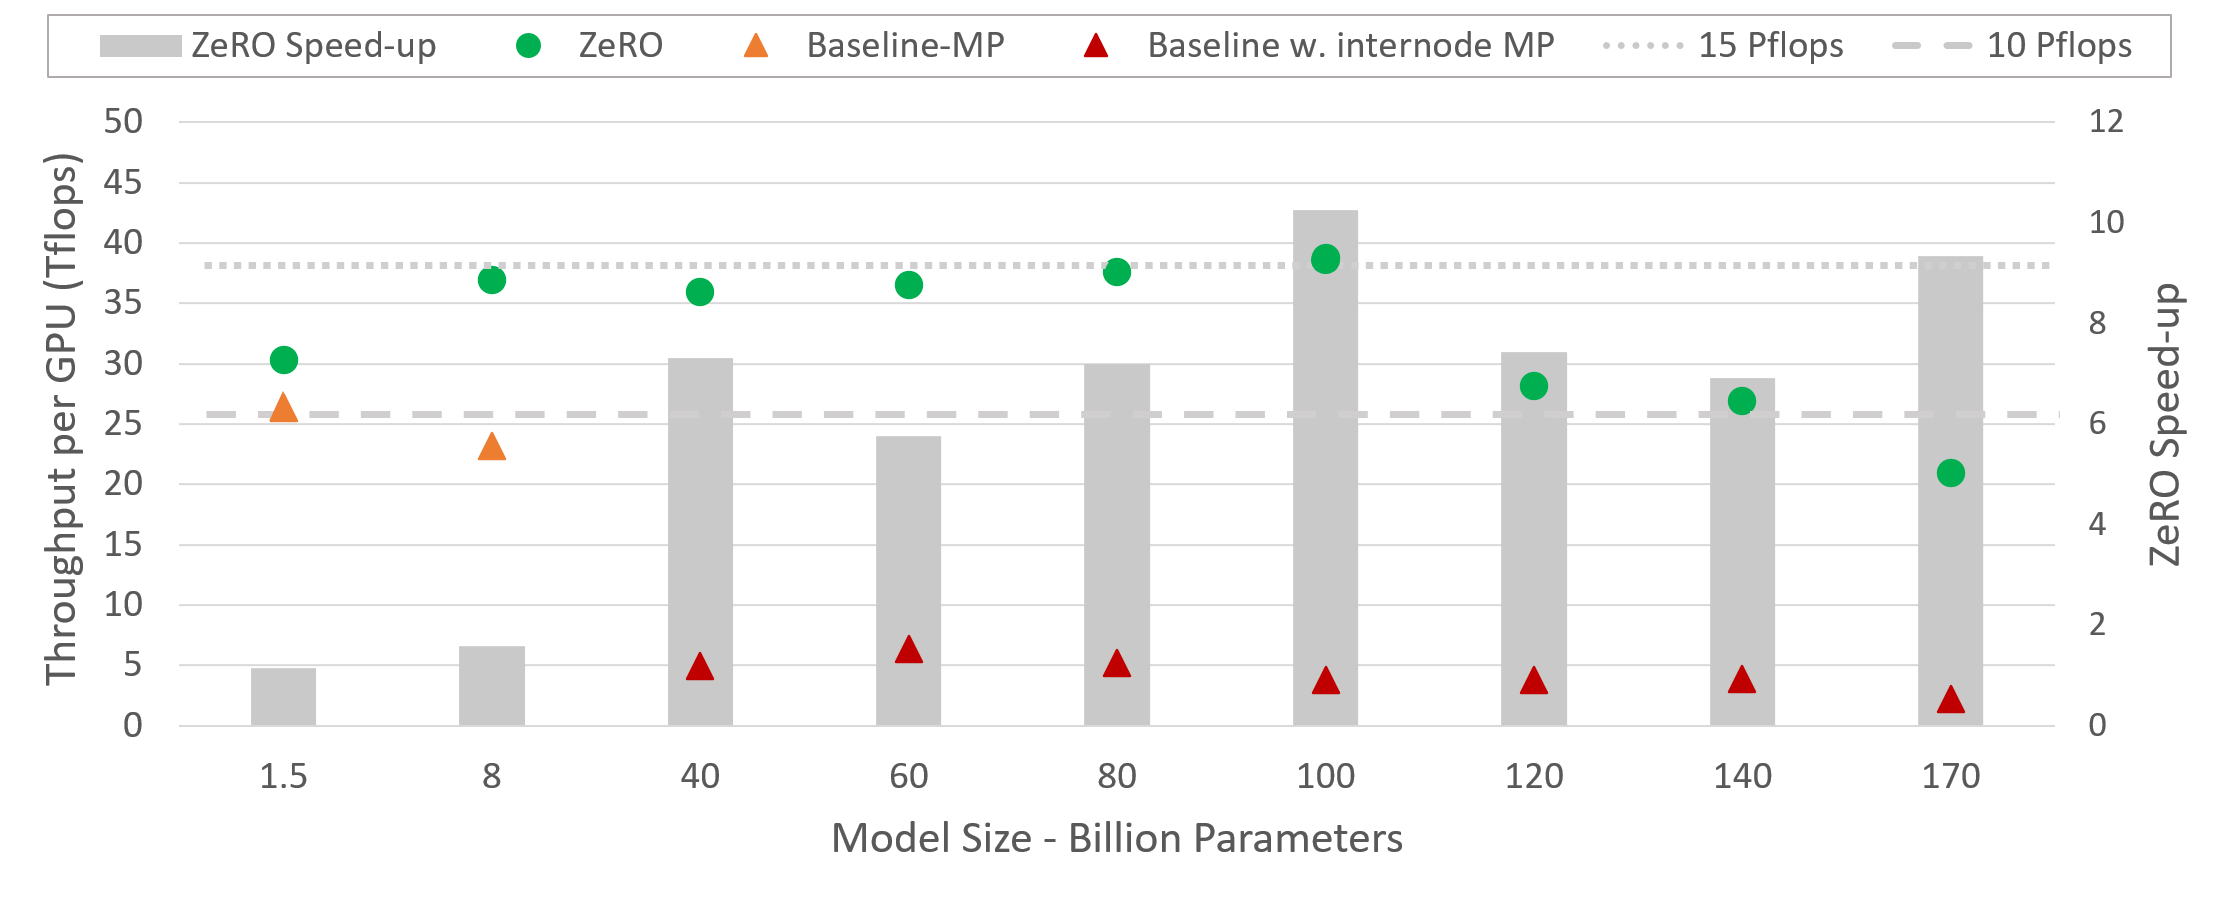
\includegraphics[width=1.0\columnwidth]{model_size_and_speedup.PNG}
   \caption{\name training throughput and speedup w.r.t SOTA baseline for varying model sizes.  For \name, the MP always fit in a node, while for baseline, models larger than 40B require MP across nodes.} 
   \label{fig:billion_parameter_speedup}
   \end{center}
\end{figure}

For \name-100B, the slight reduction in performance beyond 100B is due to lack of enough memory to run larger batch sizes.

\subsection{Super-Linear Scalability}
\name-100B demonstrates super-linear scalability for very large model sizes. Figure~\ref{fig:hyperscale_60B} shows scalability results for a 60B parameter model going from 64 to 400 GPUs and we expect this trend to continue further for more GPUs.

\begin{figure}[t!]
   \begin{center}
   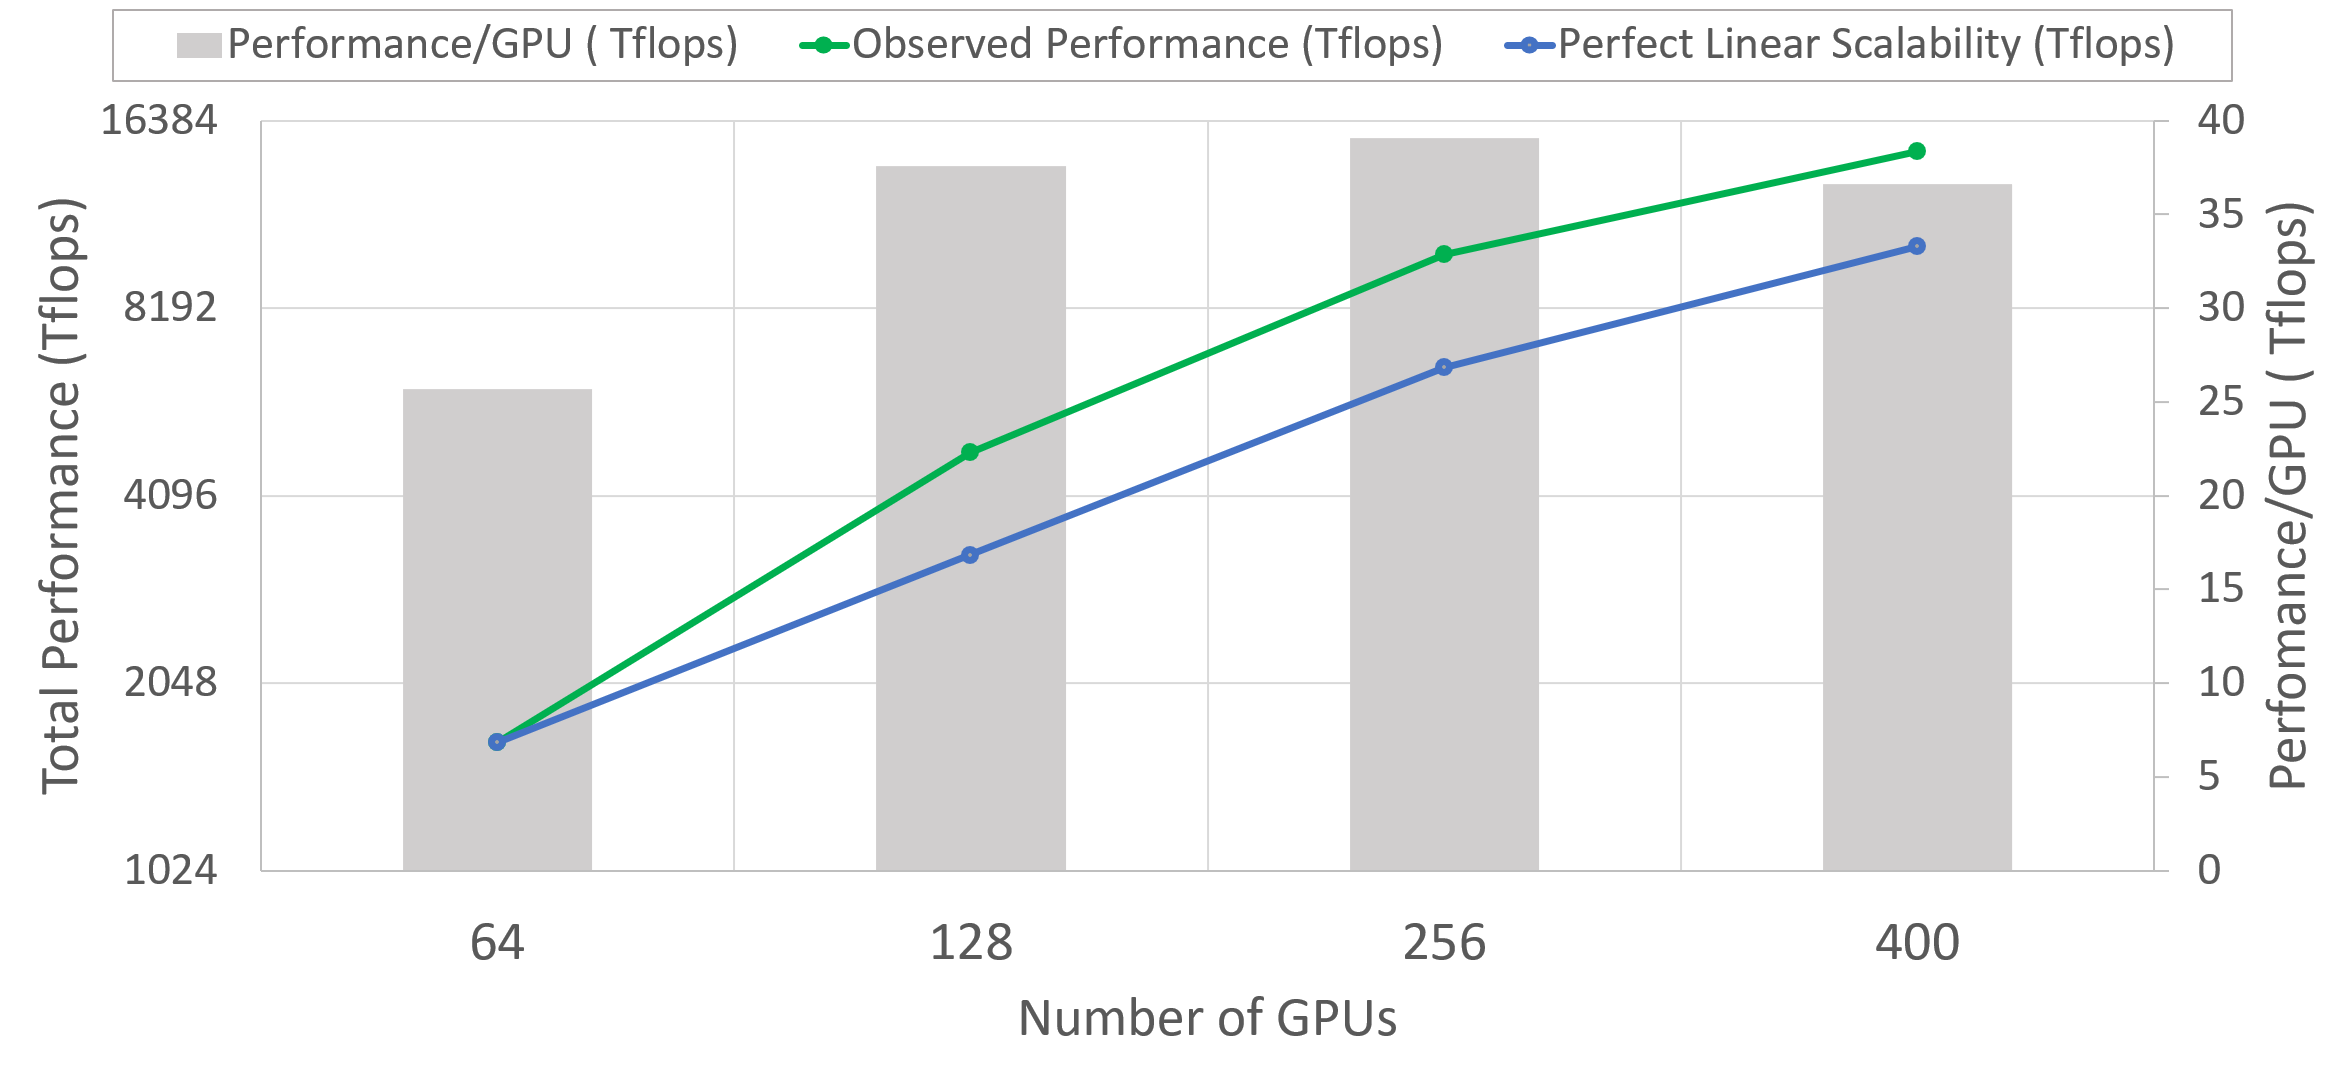
\includegraphics[width=1.0\columnwidth]{hyperscale_60B_model_v2.PNG}
   \caption{Superlinear scalability and per GPU training throughput of a 60B parameter model using \name-100B.} 
   \label{fig:hyperscale_60B}
   \end{center}
\end{figure}

\subsection{Democratizing Large Model Training}
Figure~\ref{fig:dp_tput} shows that \name-100B can train models with up to 13B parameters without MP on 128 GPUs, achieving throughput over 40\,TFlops per GPU on average.

\begin{figure}
   \begin{minipage}[b]{0.55\columnwidth}
    \centering
       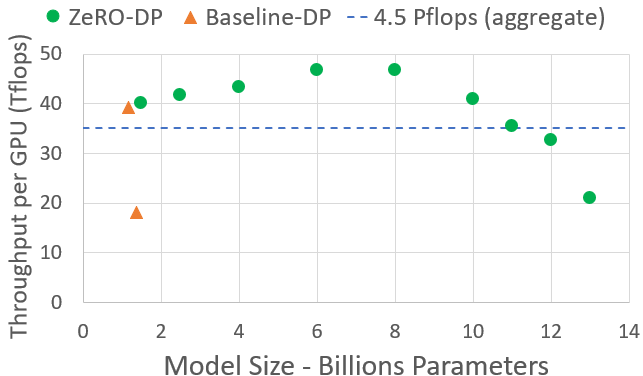
\includegraphics[width=\textwidth]{max_data_parallel_throughput.PNG}
        \caption{Max model throughput with \name-DP.} \label{fig:dp_tput}
   \vspace{0.04in}
   \end{minipage}
   \quad
   \begin{minipage}[b]{0.4\columnwidth}
    \centering
       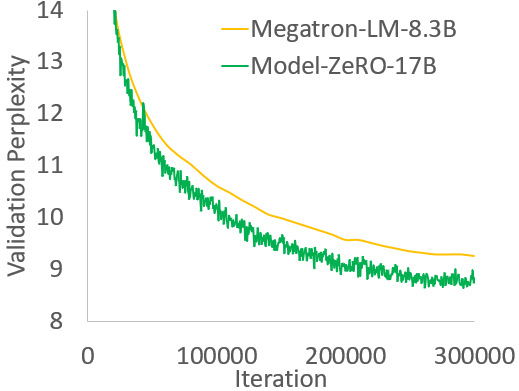
\includegraphics[width=\textwidth]{turing_nlg_17B.PNG}
        \caption{SOTA Turing-NLG enabled by \name.} \label{fig:turing_nlg_17B}
      \vspace{0.08in}
   \end{minipage}
\end{figure}

\subsection{Turing-NLG, the SOTA language model with 17B parameters}
Turing-NLG was trained end-to-end using \name-100B and Figure~\ref{fig:turing_nlg_17B} shows the validation perplexity over 300K iterations compared to previous SOTA, Megatron-LM 8.3B parameter model.

\bibliographystyle{unsrt}
\bibliography{references}

\newpage
\appendix
This is because the total number of GPUs must be a product of the number of MP, and we only had access to a total of 400 GPUs. There exist a handful of additional constraints in model configuration values, such as hidden size must be divisible by attention heads, hidden size divisible by MP, and attention heads divisible by MP.

\end{document}